\chapter{Примеры работы ПО}

В качестве примера будет рассмотрена обработка одной из веб-страниц сайта \url{chiefs.kz}. На рисунке~\ref{examplepage} изображена веб-страница в браузере.

\begin{figure}[h!]
    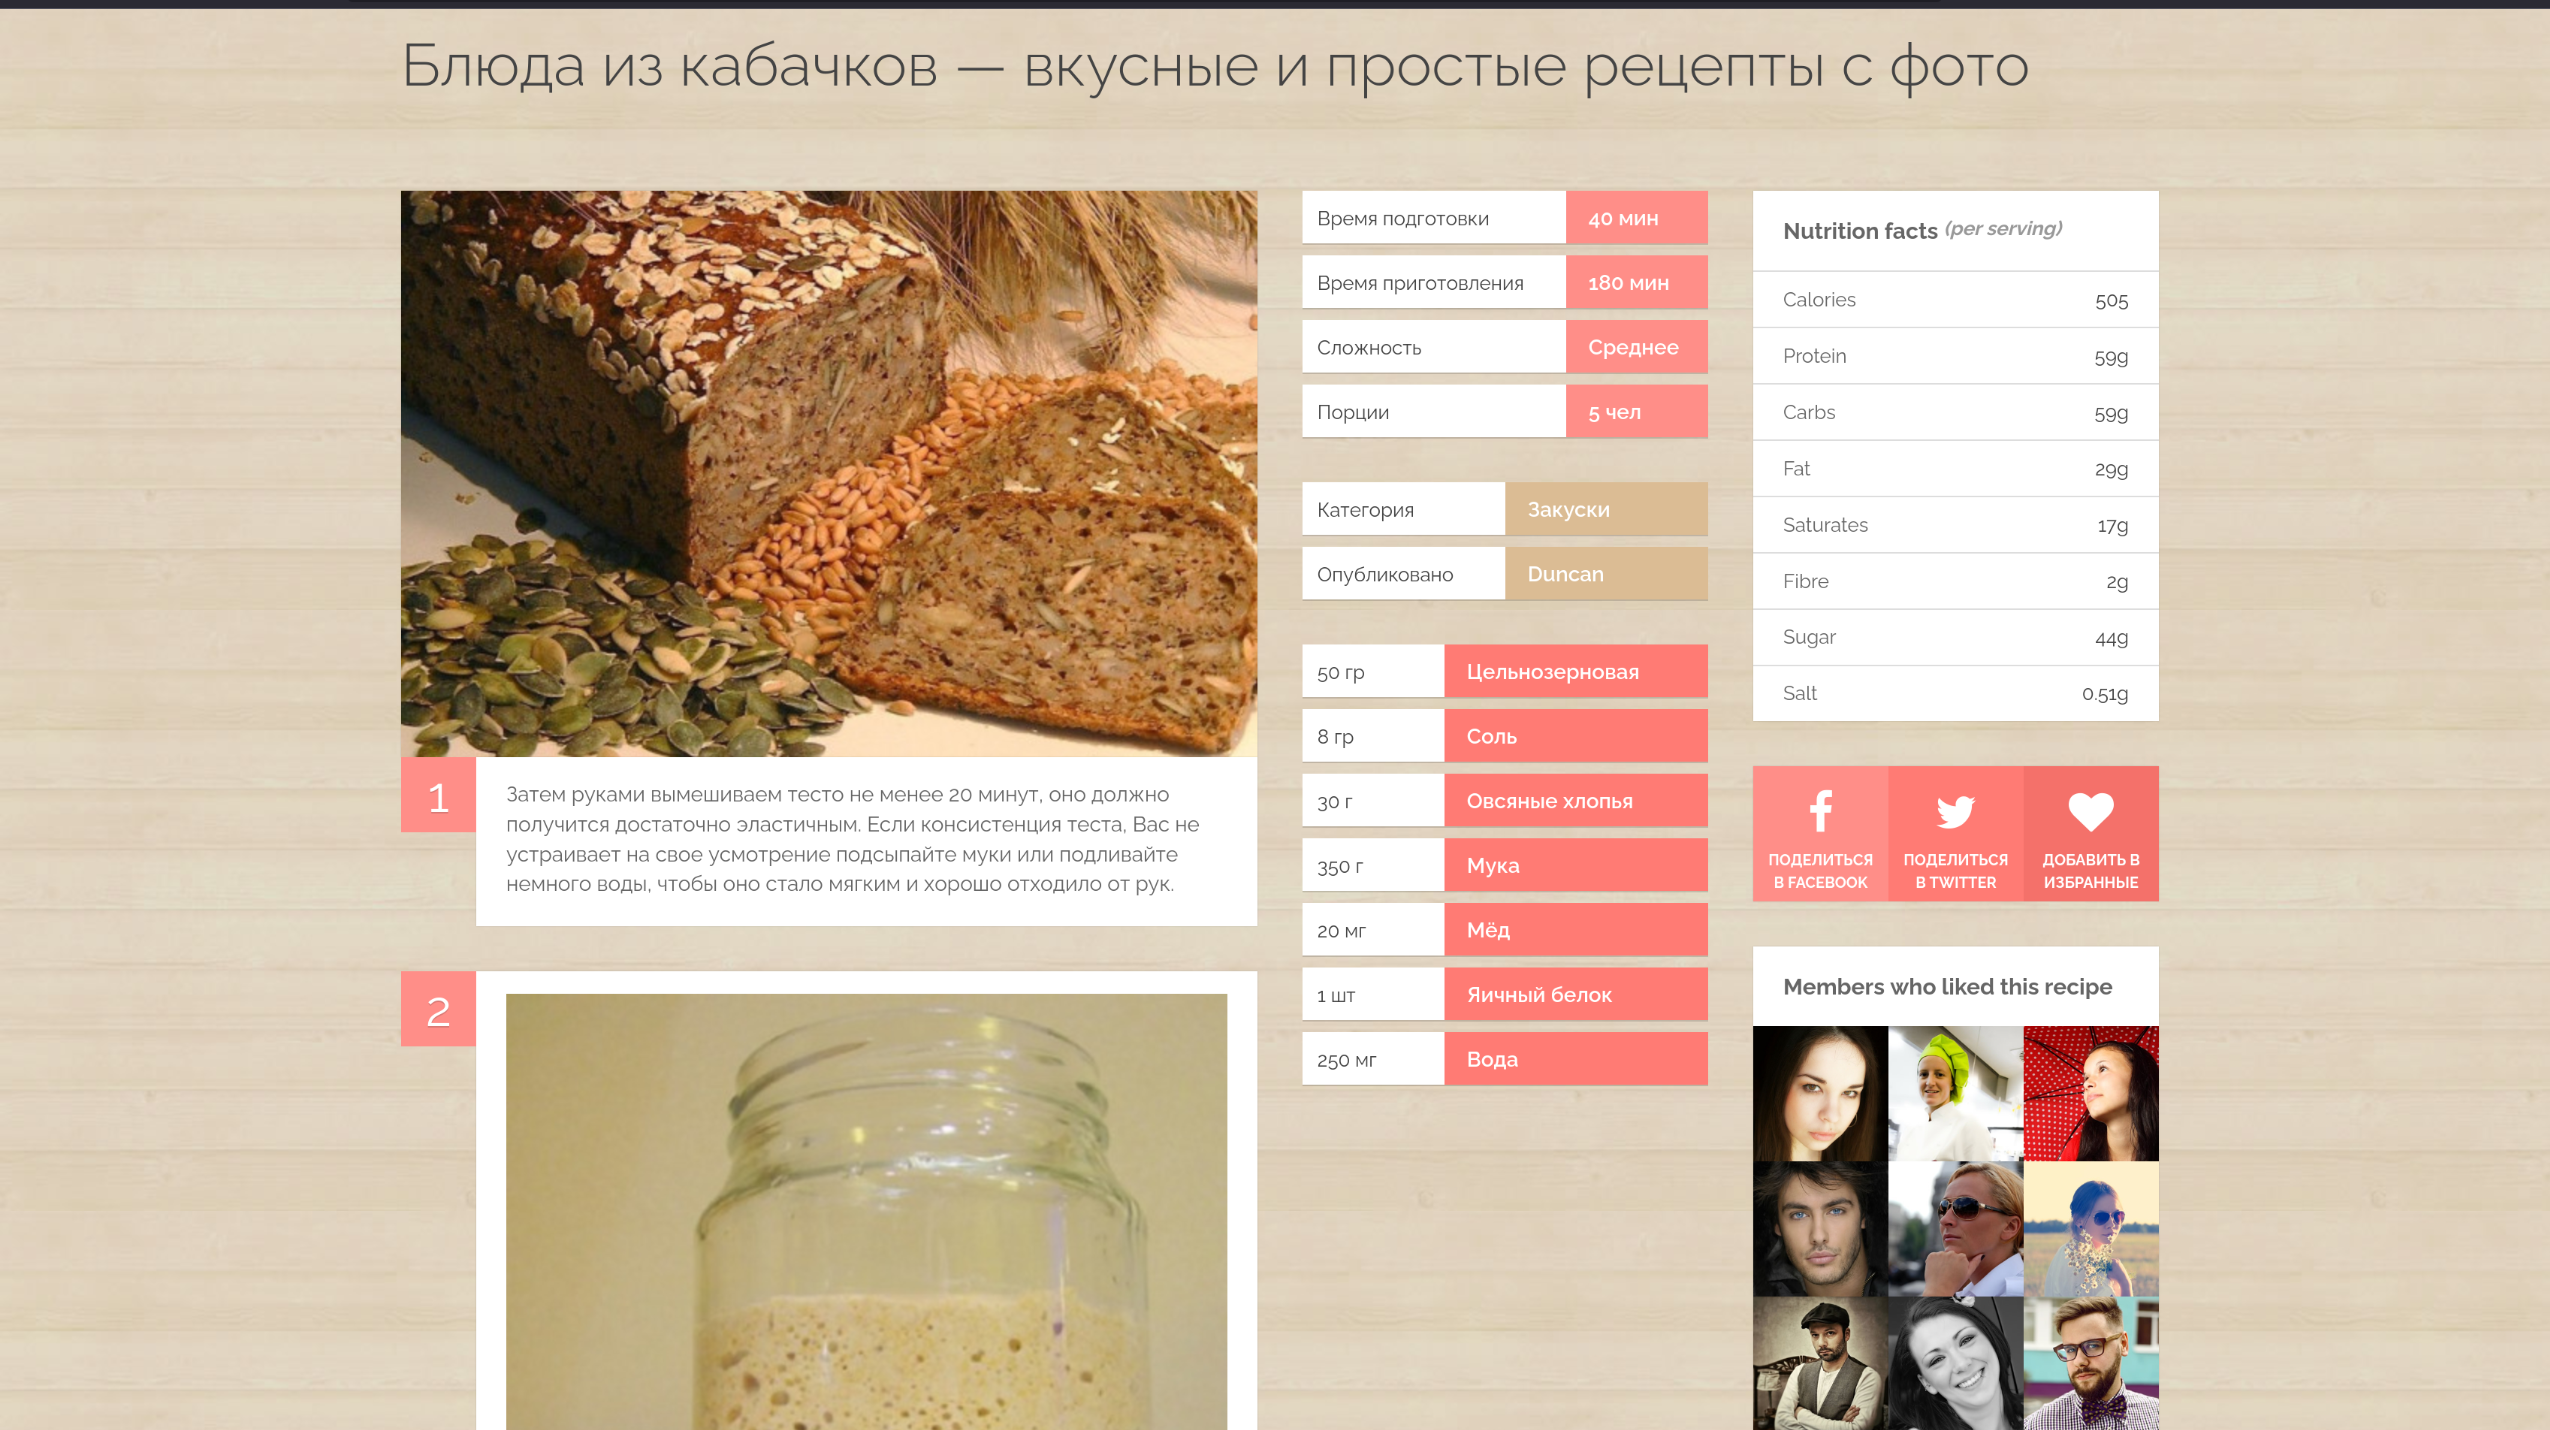
\includegraphics[width=\textwidth]{example}
    \caption{Скриншот одной из веб-страниц сайта}
    \label{examplepage}
\end{figure}

json-файл, полученный после обработки алгоритмом представлен в листинге~\ref{lst:result};

\begin{lstlisting}[caption={json-файл, полученный после обработки рецепта},label={lst:result}]
{
    "id": 4,
    "image_url": "chiefs.kz/img/0/2061.jpg",
    "ingredients": "{[{\"name\":\"Цельнозерновая\",\"quantity\":\"50 гр\"},{\"name\":\"Соль\",\"quantity\":\"8 гр\"},{\"name\":\"Овсяные хлопья\",\"quantity\":\"30 г\"},{\"name\":\"Мука\",\"quantity\":\"350 г\"},{\"name\":\"Мёд\",\"quantity\":\"20 мг\"},{\"name\":\"Яичный белок\",\"quantity\":\"1 шт\"},{\"name\":\"Вода\",\"quantity\":\"250 мг\"},]}",
    "issue_id": 9185,
    "steps": "1: Затем руками вымешиваем тесто не менее 20\nминут, оно должно получится достаточно\nэластичным. Если консистенция теста, Вас не\n устраивает на свое усмотрение подсыпайте муки\nили подливайте немного воды, чтобы оно\nмягким и хорошо отходило от рук.\n2: В одной порции пшеничной закваски около 50\nграмм, это нужное количество для приготовления\nзакваски используемой цельнозерновую муку. Для\nприготовления такой опары, добавляем в готовую\nпшеничную закваску 50 грамм теплой воды и такое\nже количество цельнозерновой муки и даем\nнастояться и подняться.\n 3: Из полученной порции опары и будем готовить наш\n хлеб.\n4: Для этого все ингредиенты смешиваем воедино,\nисключая яичный белок и овсяные хлопья, они\nбудут участвовать в завершительном процессе\nприготовления. Смесь пока особо не вымешиваем,\nоставляем на полчаса.\n",
    "title": "Блюда из кабачков - вкусные и простые рецепты с фото"
},
\end{lstlisting}
